% Appendix A

\chapter{Sample FAST Simulation Input Files} % Main appendix title

\label{AppendixA} % For referencing this appendix elsewhere, use \ref{AppendixA}

\lhead{Appendix A. \emph{Sample FAST Simulation Input Files}} % Change X to a consecutive letter; this is for the header on each page - perhaps a shortened title

The following pages contain samples of the \textit{primary.fst} and \textit{Aerodyn.ipt} FAST input files. Many FAST simulations were run in this dissertation and some settings varied from one simulation to another, but the parameters shown in these input files illustrate typical settings used in this dissertation. FAST also uses input files to specify the wind flow field, the structural properties of the turbine tower,  and the structural and aerodynamic properties of the turbine blades. Those other input files have not been included here because they are either dictated by the properties of the NREL 5-MW turbine, or they are generated by another simulation tool.

\pagebreak
\section{primary.fst} \label{sectionA-1}

\noindent
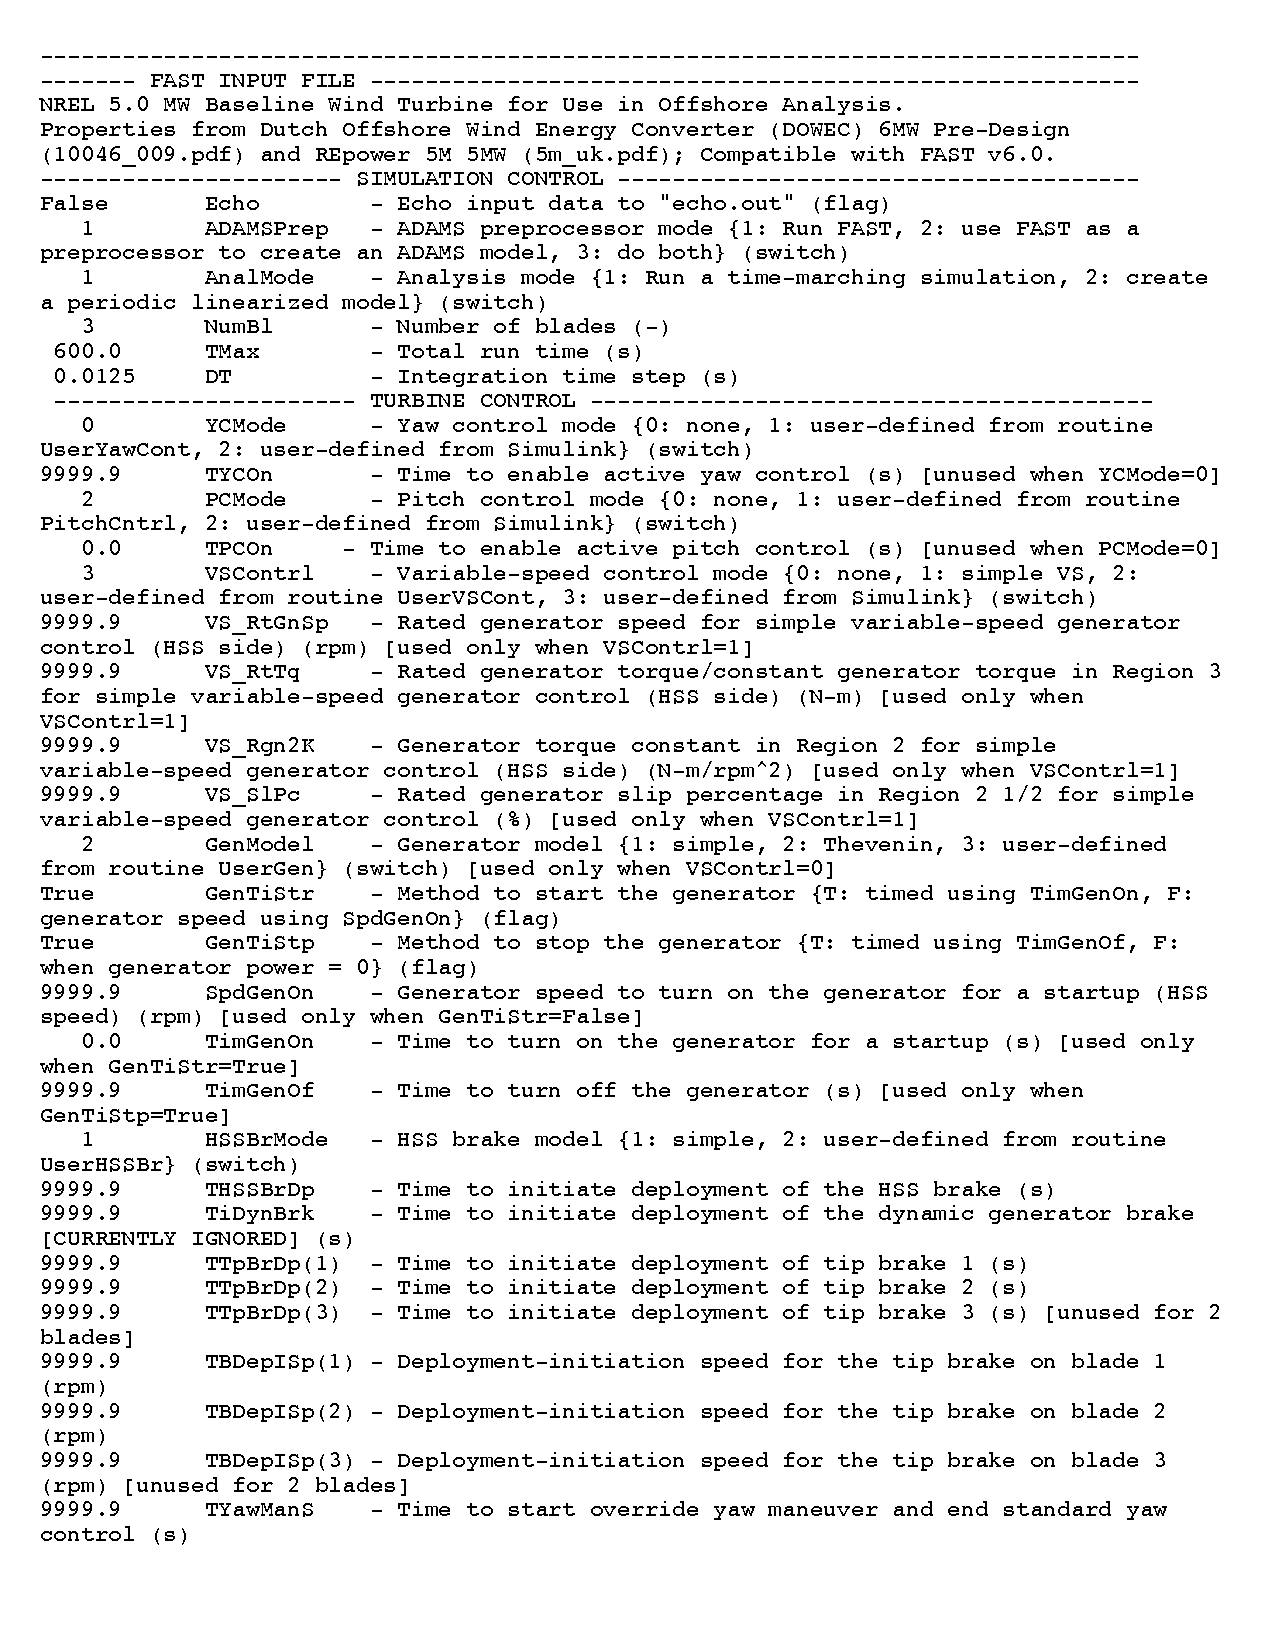
\includegraphics[width=\linewidth]{Figures/AppendixAFigures/primaryP1.pdf}		

\noindent
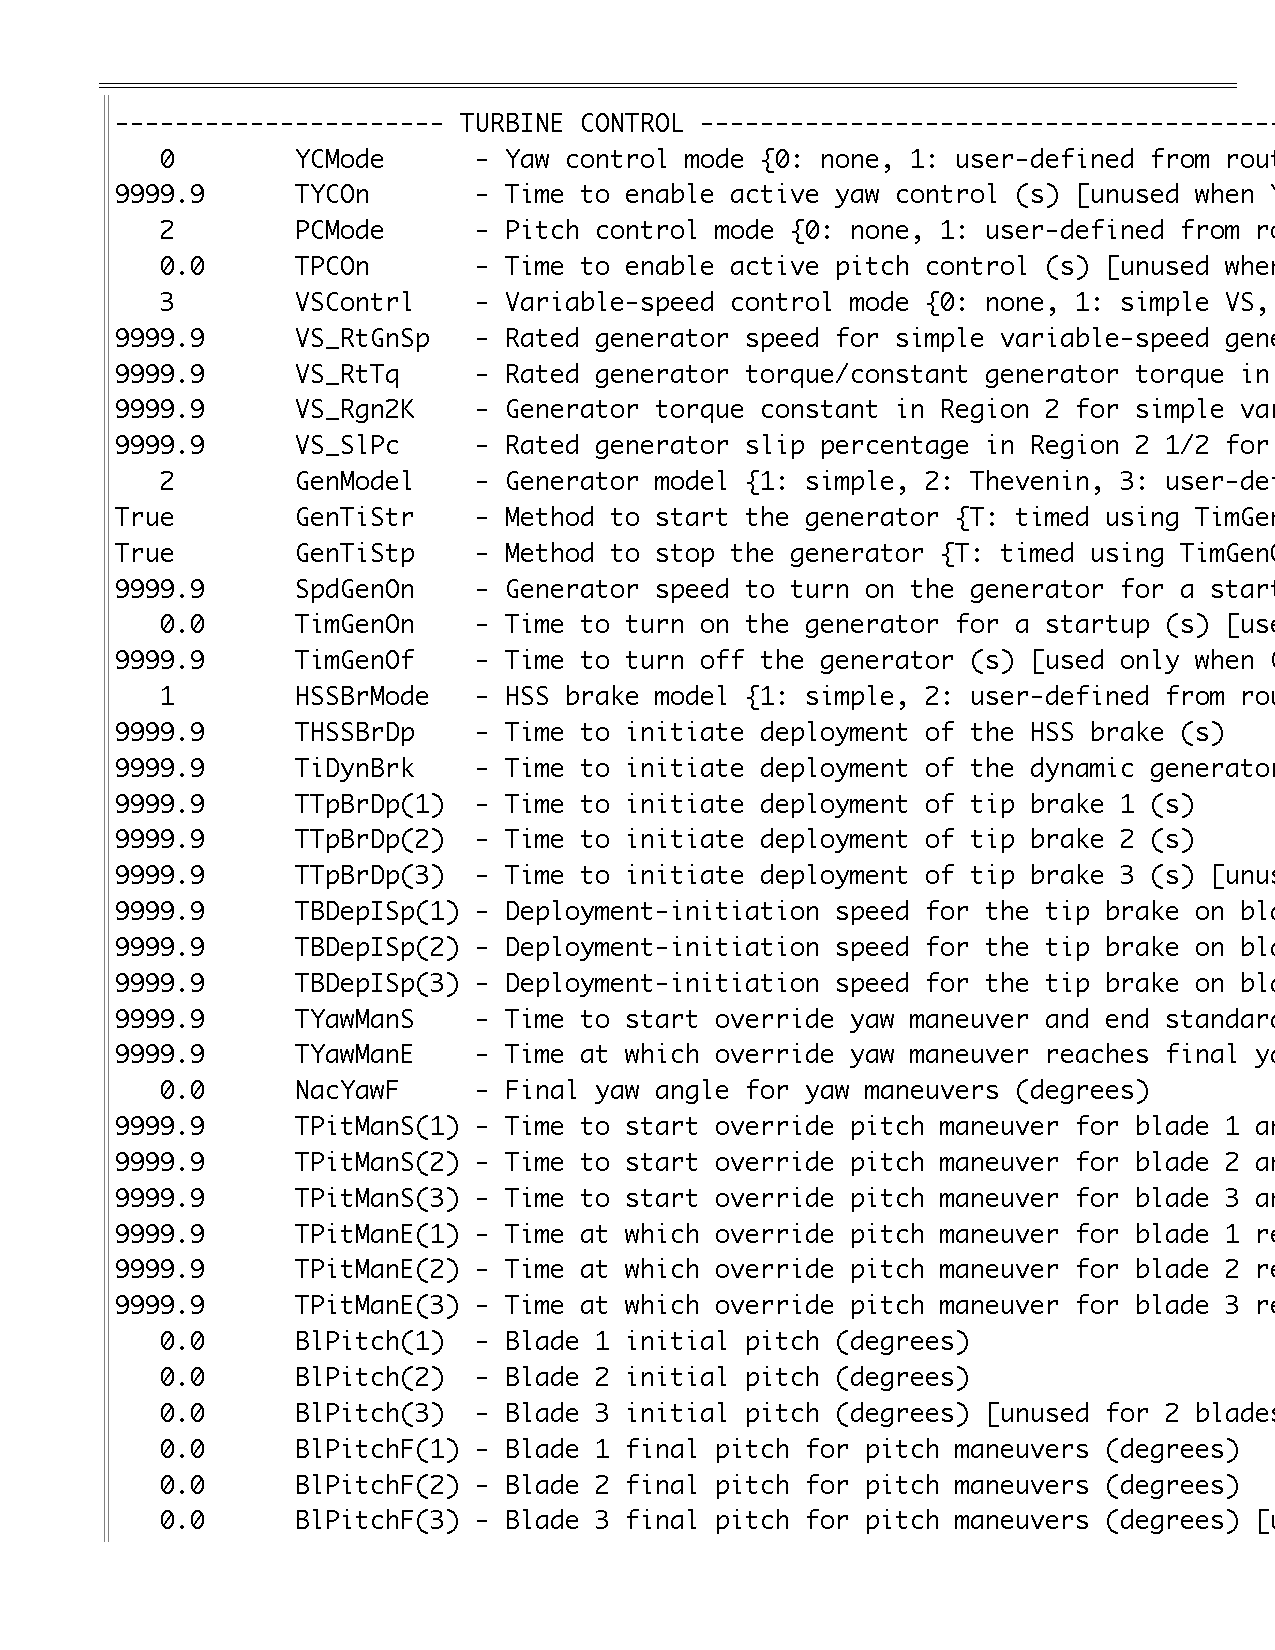
\includegraphics[width=\linewidth]{Figures/AppendixAFigures/primaryP2.pdf}

\noindent
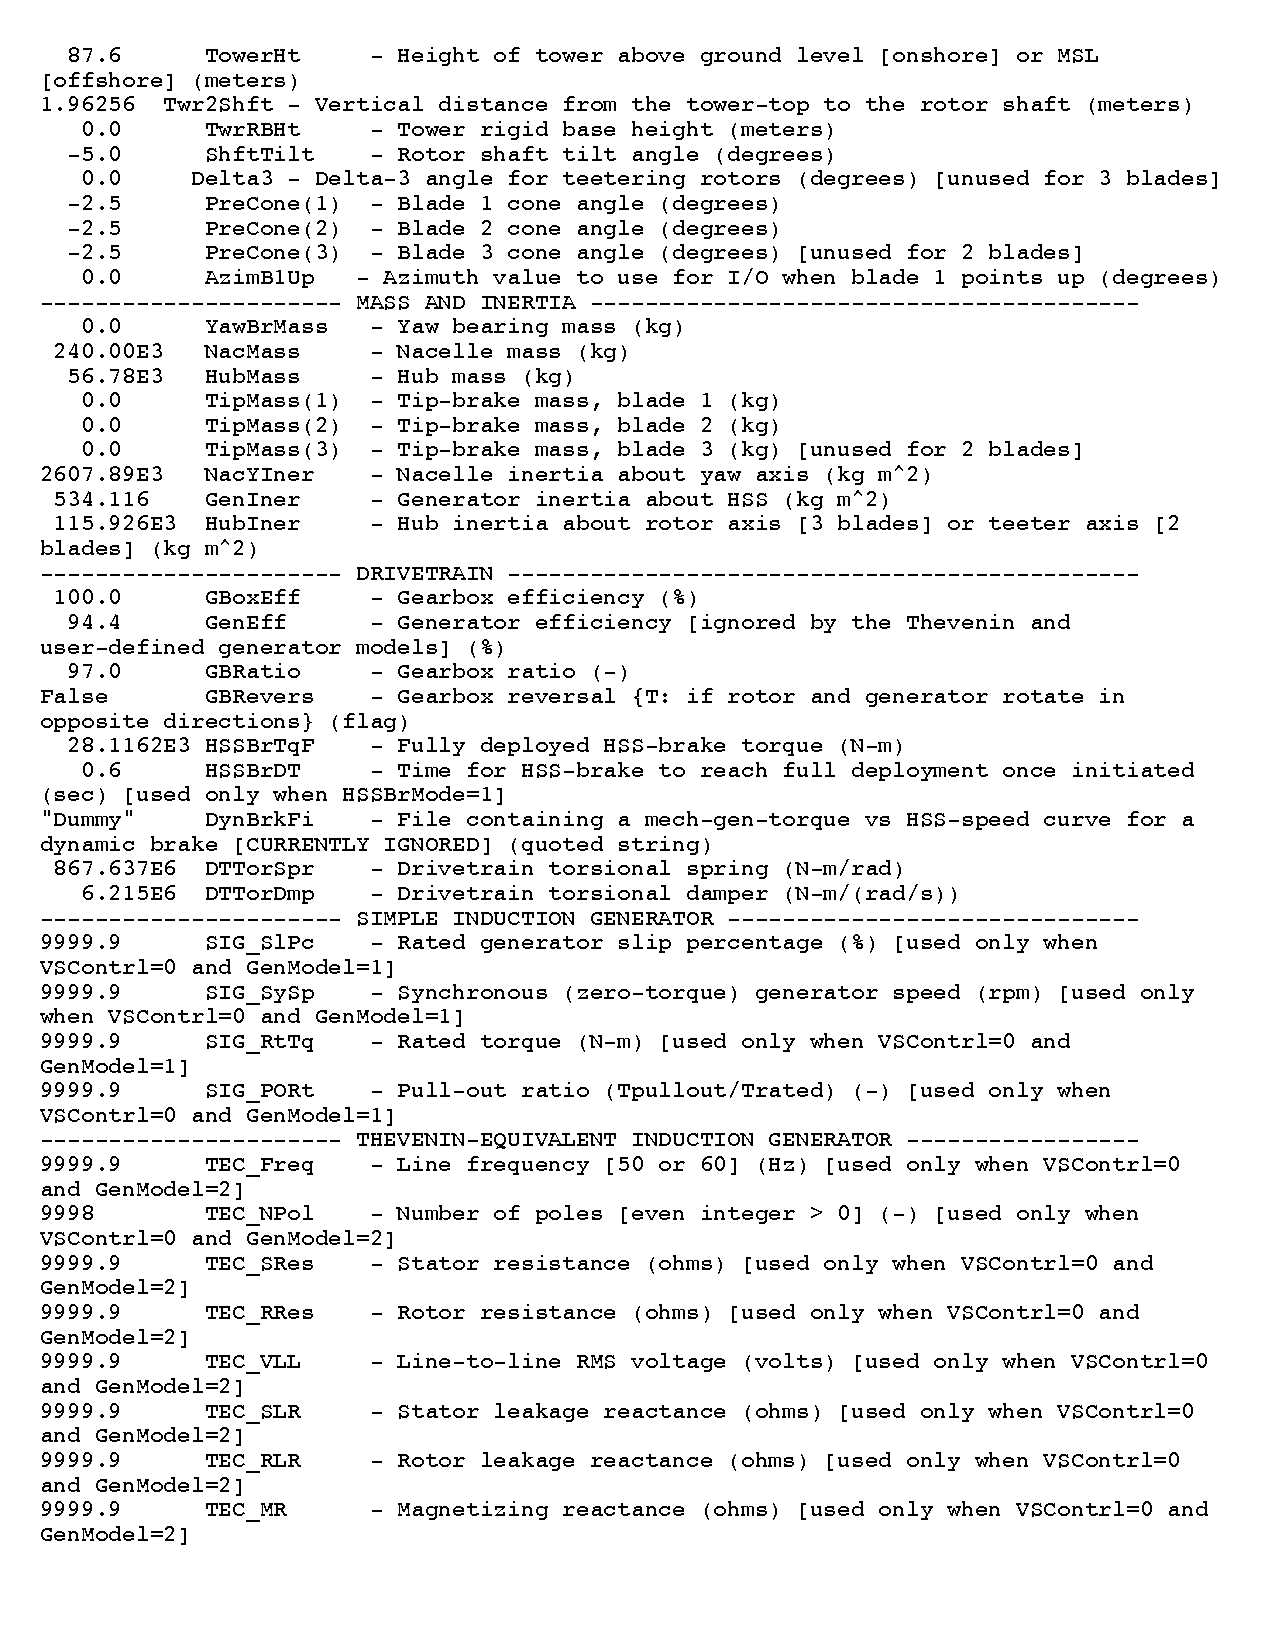
\includegraphics[width=\linewidth]{Figures/AppendixAFigures/primaryP3.pdf}	

\noindent
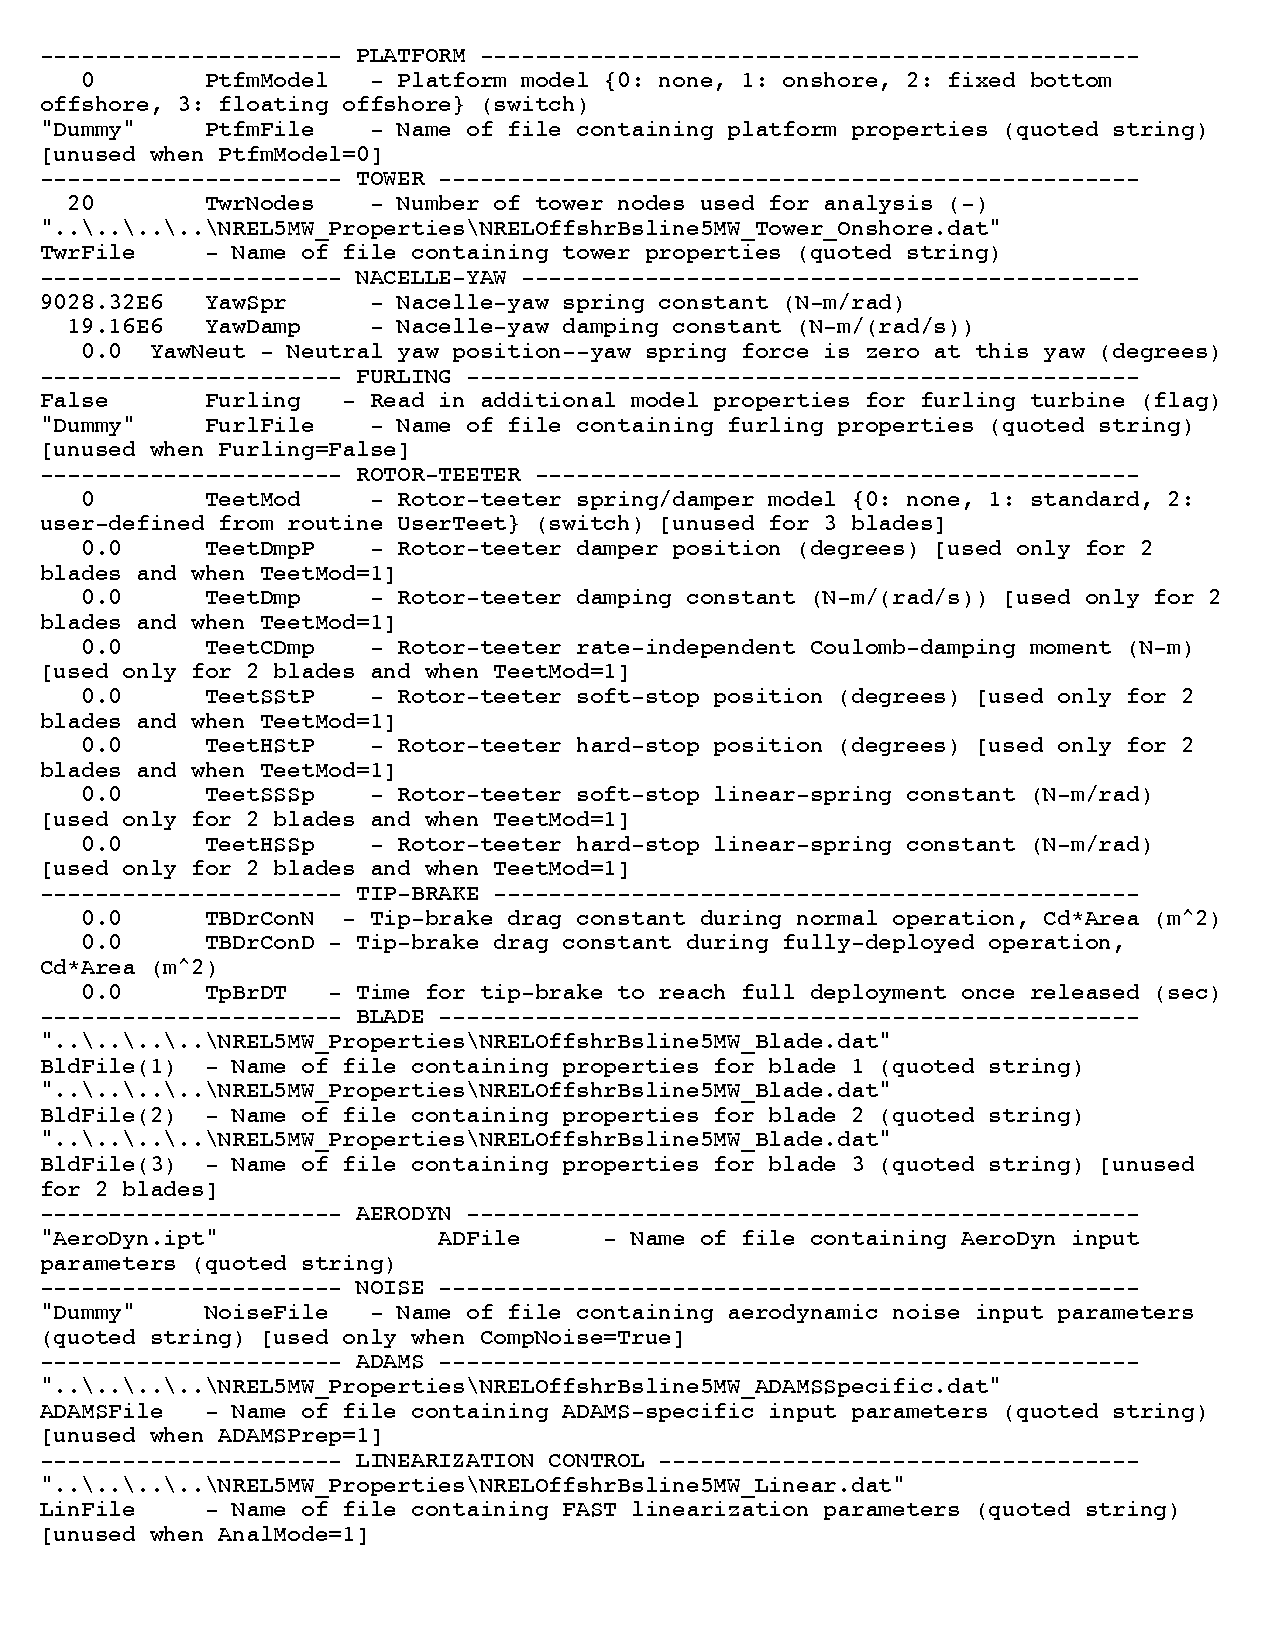
\includegraphics[width=\linewidth]{Figures/AppendixAFigures/primaryP4.pdf}	

\noindent
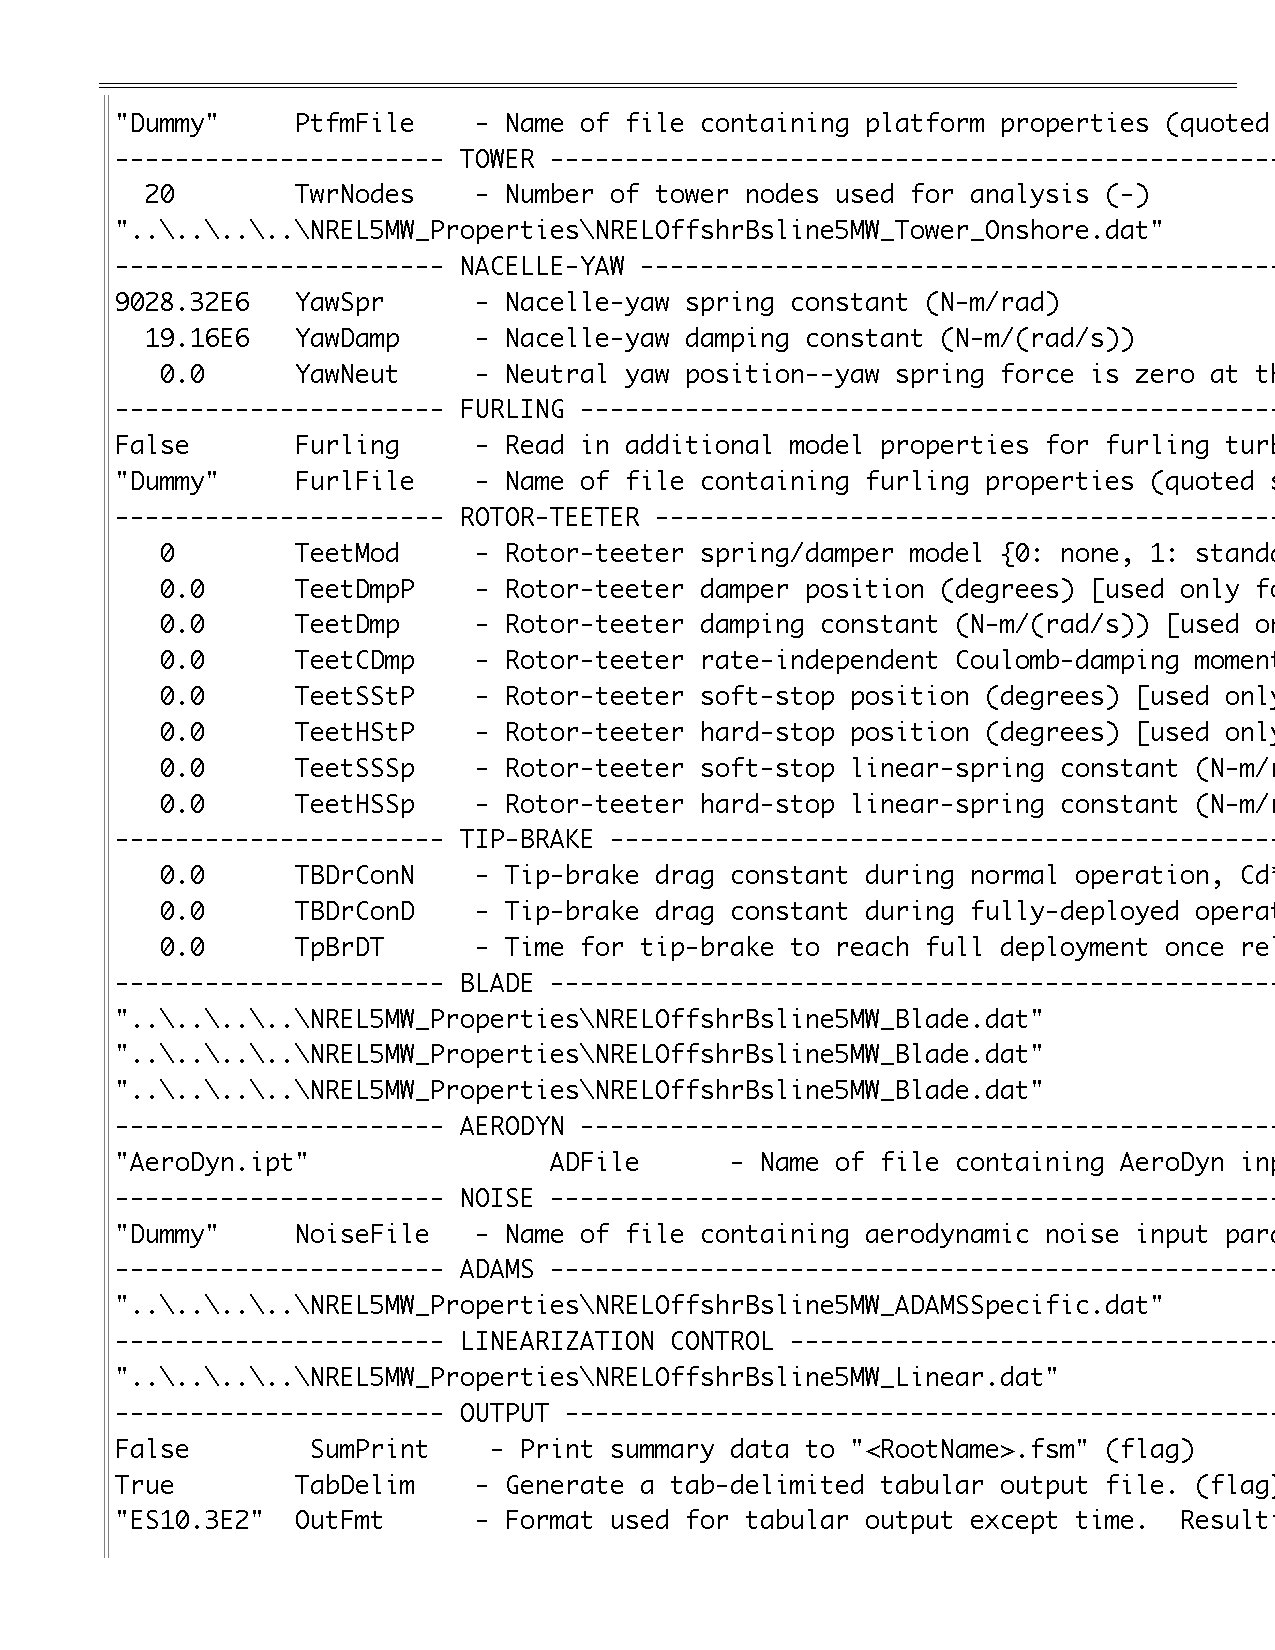
\includegraphics[width=\linewidth]{Figures/AppendixAFigures/primaryP5.pdf}	



\section{Aerodyn.ipt} \label{sectionA-2}

\noindent
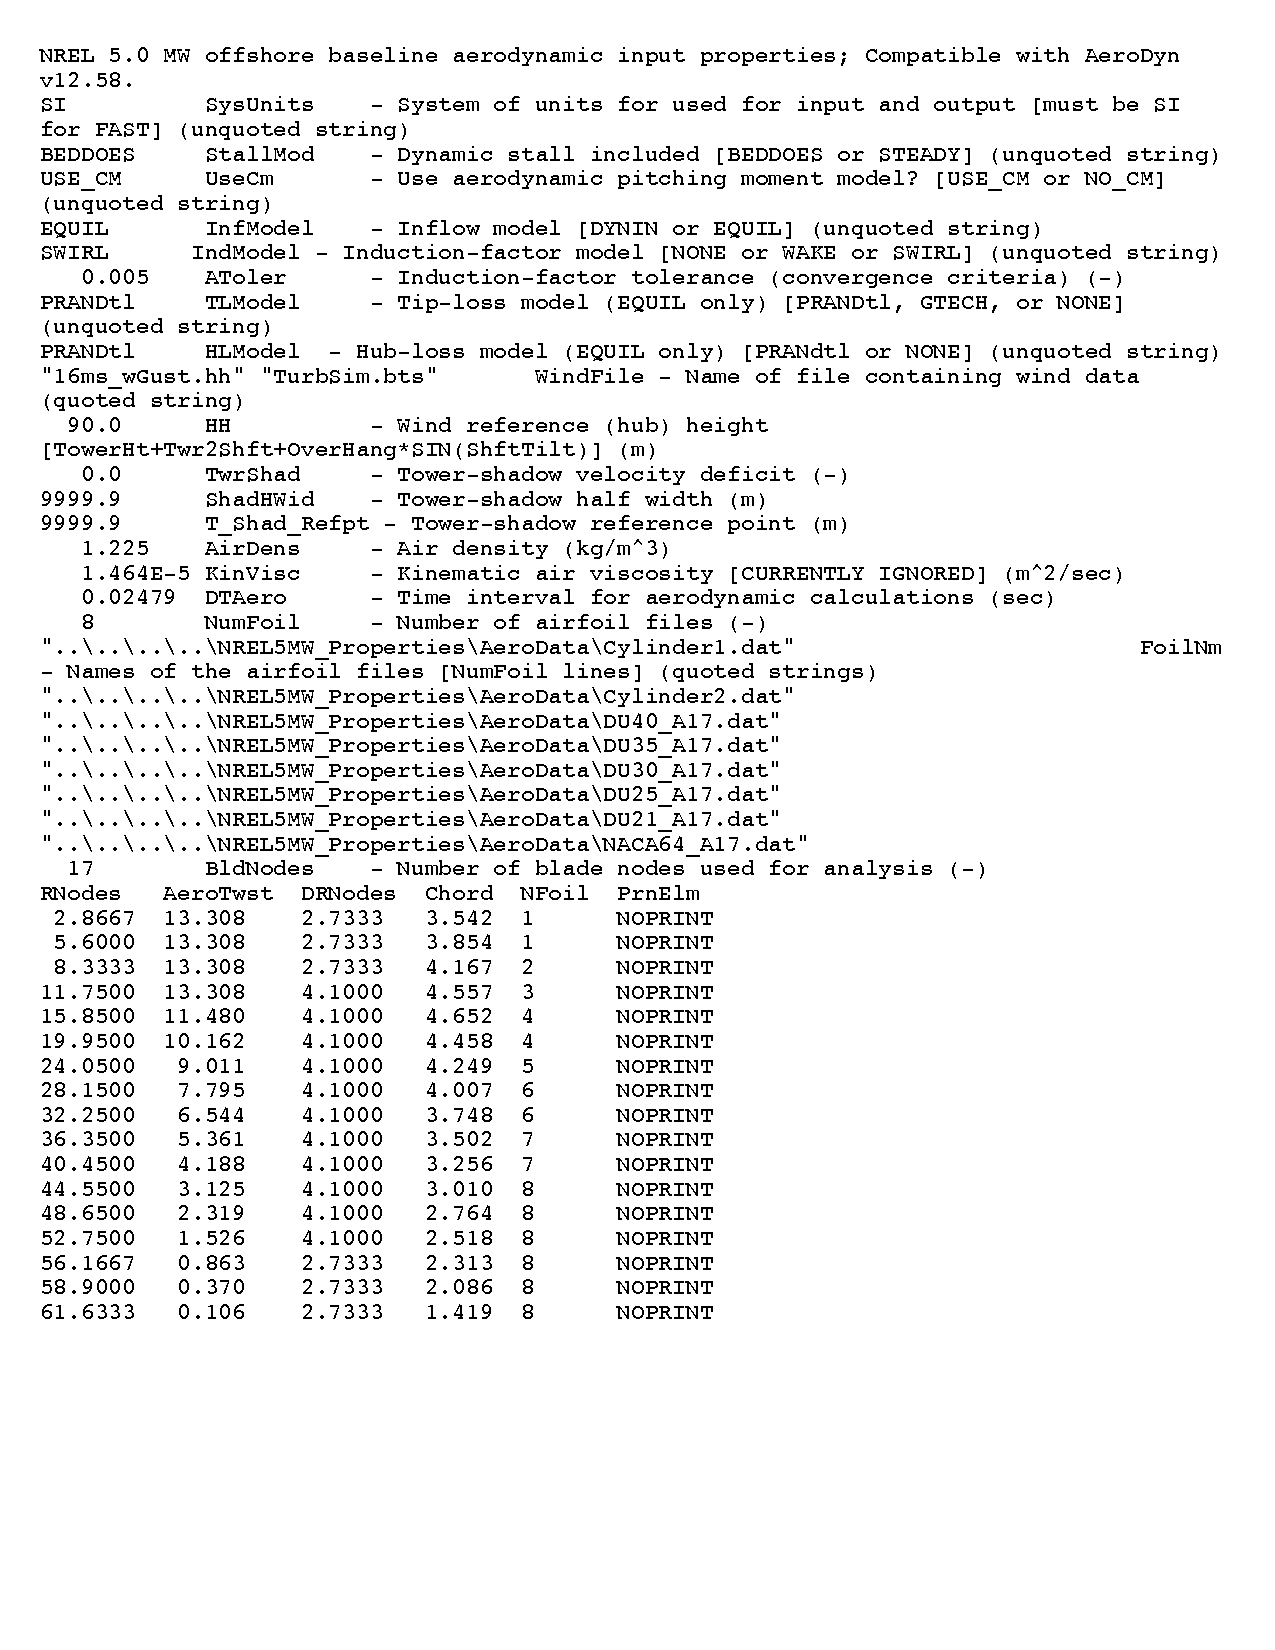
\includegraphics[width=\linewidth]{Figures/AppendixAFigures/aerodyn.pdf}		
